\documentclass{article}

% Language setting
% Replace `english' with e.g. `spanish' to change the document language
\usepackage[english]{babel}

% Set page size and margins
% Replace `letterpaper' with `a4paper' for UK/EU standard size
\usepackage[letterpaper,top=1cm,bottom=1cm,left=2cm,right=2cm,marginparwidth=1.75cm]{geometry}

% Useful packages
\usepackage{amsmath}
\usepackage{graphicx}
\usepackage[colorlinks=true, allcolors=blue]{hyperref}
\usepackage[
backend=biber,
style=alphabetic,
sorting=ynt
]{biblatex}
\usepackage{csquotes}
\usepackage{listings}
\usepackage{color}
\lstloadlanguages{C,C++,csh,Java}

\addbibresource{references.bib}

\title{Analysis of Post Quantum Cryptography and Comparison of Quantum Key Distribution mechanisms}
\author{Lee Dale}

\begin{document}
\maketitle

\section{Introduction}

At some point in the future quantum computers will have enough processing power or Qubits to successfully implement quantum algorithms that can break the encryption of our current state of the art public key exchange mechanisms \cite{Bellizia2021Post-QuantumDesign}. Once this happens there will be a need for robust quantum key exchange methods that allow privacy of message exchange to be maintained, even when subjected to a quantum computing algorithms. 

This paper outlines the current weaknesses in public key exchange methods that rely on the a mathematically hard to compute private key and why these will be vulnerable to quantum computers. It will then outline some key solutions to this problem that will be robust in a post quantum world. 

\section{Literature Review}

\subsection{Overview of current key exchange mechanisms}
As it stands most communication methods used over the internet rely on asymmetric cryptography

The methods currently available to us for key exchange fall into three main categories that all rely on the premise that there is publicly available information used for the key exchange between two parties and there is also private information only known to the individual. The secrecy of the public key exchange relies on the fact  that it is hard to compute using a typical Turing state machine approach of classical computers. 

Anderson mentions \cite{AndersonR2020} "The technique is to make the security of the cipher depend on the difficulty of solving a certain mathematical problem. The two problems which are used in almost all fielded systems are factorization (used in most commercial systems) and discrete logarithm (used in many government systems)." 

I have broken discrete logarithms into two categories, with the addition of discrete logarithms that use elliptic curves. These are outlined below.

\subsubsection{Prime Factorization}

In the RSA method of cryptography, prime factorization is used as the basis for the algorithm's security. The RSA algorithm works by selecting two large prime numbers, p and q, and multiplying them together to obtain a product, $n = p*q$. This product n is then used as the modulus for the public and private keys.

The security of RSA relies on the fact that it is difficult to factorize the large composite number n back into its two prime factors, p and q. Specifically, if someone knows the value of n, it is difficult for them to find p and q without trying all possible factors, which becomes computationally infeasible for large enough values of p and q.

The private key in RSA cryptography is derived from the factors p and q of n, which are kept secret. The public key, on the other hand, is the modulus n and an exponent e, which is typically a small odd integer such as 3 or 65537.

To encrypt a message using RSA, the message is first converted into a number and then raised to the power of the public exponent e modulo n. The resulting ciphertext can only be decrypted using the private key, which involves factoring the modulus n back into its two prime factors p and q.

Thus, prime factorization plays a crucial role in the security of RSA cryptography. The larger the prime factors used in the algorithm, the more secure it is against attacks that attempt to factorize the modulus n.

\subsubsection{Discrete Logs}
Discrete logarithms are used in various public key cryptography algorithms, such as Diffie-Hellman key exchange, ElGamal encryption, and digital signature schemes like the Digital Signature Algorithm (DSA) and Schnorr signature.

In these algorithms, the difficulty of computing discrete logarithms in certain mathematical groups is exploited to provide security guarantees.

In the context of public key cryptography, the groups used are typically finite fields or elliptic curves, and the discrete logarithm problem refers to the challenge of finding the exponent required to generate a given element of the group from a fixed base element.

For instance, in the Diffie-Hellman key exchange protocol, two parties agree on a shared group, a generator of that group, and publicly exchange their exponentiations of the generator. The shared secret key is computed from their respective exponentiations, which are then equal to each other, but difficult for an attacker to determine without knowledge of the secret exponents.

The discrete logarithm problem is a key component of many public key cryptography algorithms, where it is used to provide security guarantees by making it computationally infeasible for an attacker to determine a secret key from its corresponding public key.

\subsubsection{Discrete logs with Elliptic Curves}
Elliptic curve cryptography is a type of public-key cryptography that is based on the mathematics of elliptic curves. Elliptic Curve Diffie-Hellman (ECDH) is an example of a public key exchange based on elliptic curves and is widely used in web browsers.

In ECDH, two parties, say Alice and Bob, first agree on a publicly known elliptic curve E over a finite field F. They also choose a base point P on the curve, which is also publicly known.

Each party, Alice and Bob, then chooses a secret integer, which is kept private. Alice's secret integer is denoted by a and Bob's secret integer is denoted by b. They use these secret integers to compute their respective public keys as follows:

Alice computes her public key A = aP on the elliptic curve E.
Bob computes his public key B = bP on the elliptic curve E.
Alice and Bob then exchange their public keys A and B over an insecure channel.

Once Alice and Bob have exchanged their public keys, they can derive a shared secret key using the following steps:

Alice computes the point Q = aB on the elliptic curve E.
Bob computes the point Q' = bA on the elliptic curve E.
The shared secret key is then derived from the x-coordinate of the point Q (or Q') using a one-way hash function.

The security of ECDH comes from the fact that it is difficult to compute the private keys a and b from the public keys A and B, even if the elliptic curve E and the base point P are known.

ECDH allows two parties to derive a shared secret key without revealing their private keys over an insecure channel, and its security is based on the difficulty of computing discrete logarithms on the elliptic curve.

\subsection{How current mechanisms are vulnerable to quantum computers}
In a 1984 paper David Deutch \cite{Deutsch1985QuantumComputer} discussed a universal quantum computer in which he shows that a quantum computer can evolve computational basis states into linear superposition's of each other. Building on this work a decade later it was then shown by Peter Shor \cite{Shor1994AlgorithmsFactoring} that it was possible to design algorithms to factor large integer values and find discrete logarithms in polynomial time. These algorithms threaten the viability of the key exchange mechanisms discussed above and render them unusable should a quantum computer be built with enough Qubits to successfully run Shor's proposed algorithms.

It is considered that an algorithm is efficient when the number of steps grow as a polynomial to the size of its input. \cite{Shor1994AlgorithmsFactoring}  However there exists no algorithm for factoring large integers that meets this criteria based on a classical computer. Montgomery \cite{Montgomery1994AAlgorithms} states "No polynomial-time algorithm for solving this problem is known ."  Shor however in his 1994 paper  outlined  \cite{Shor1994AlgorithmsFactoring} such an algorithm that can be executed on a quantum computer that does meet this criteria. 

The issue for any asymmetric cryptography that relies on large integer factorization such as the popular RSA method is that instead of taking exponential time to find the prime factors of a large integer, a quantum computer will carry out this calculation in polynomial time. 

If we use a brute force a method that takes 2 seconds per key to try all the keys for a 4 bit encryption key using an algorithm that has exponential time complexity we get:

\[Keys = 2^4 = 16\]
\[f((2^2)^4)) = 65536\]


Instead with polynomial time we get:
\[f((2^4)^2) = 256\]

We can see the polynomial time algorithm will be much faster to brute force an integer factorization problem. The time taken will also grow less quickly with the polynomial time complexity than with the exponential time complexity.

This means with a quantum computer it will become feasible for an attacker to find out the prime factors that make up a public key in a cryptographic encryption scheme that relies on the hardness of the prime factorization problem, and by extension discrete logs. If there came a time when a quantum computer could execute Shor's algorithms for 2048 bit encryption keys, this would render all current methods for public key cryptography useless.

\subsection{Quantum robust methods}
Various methods have been devised to deal with a world where quantum computers are able to crack encryption keys up to 2048 bits long. Kumar and Garhwal state that quantum protocols are based on either the Heisenberg Uncertainty principle or quantum entanglement \cite{Kumar2021State-of-the-ArtCryptography} I will outline the most notable methods in this section and then focus on quantum key distribution based on quantum entanglement. 

\subsubsection{Lattice based cryptography}

\subparagraph{Issues}

\subsubsection{Quantum Key Distribution}
The no cloning theorem in quantum mechanics leads us to an interesting way of distributing secret keys between two parties. If we use a secret key that exists in a superposition of entangled states and subsequently share this secret key between two parties, there would always be a way to detect whether the key had been tampered with in transit. This is explained by the fact that if an eavesdropper had modified the key in any way (in quantum mechanics we say that the entangled state was observed) the secret key would have de-cohered into one of the many possible superposition of states and therefore each party would be able to detect the eavesdroppers attempt at intercepting the secret key. 

\subsubsection{Quantum key distribution using entangled photons}
From Kumar and Garhwal \cite{Kumar2021State-of-the-ArtCryptography} quantum key distribution protocols are classified into two categories; Discrete variable QKD and Continuous variable QKD. Discrete variable QKD is based around the spin of an electron or the polarization of a single photon. Continuous variable QKD is mainly based around the use of a laser to store information in the form if a continuous light source.

We will concentrate here on a discrete variable QKD example in the BB84 protocol which uses the polarization of single photons.  

The BB84 protocol was first introduced by Charles Bennet and Gilles Brassard in 1984 \cite{Bennett2020QuantumTossing} . In the BB84 protocol the two parties, say Alice and Bob establish two communication channels. The first is a classical communication channel that conforms to the laws of classical physics and the second is a quantum communication channel which conforms to the laws of quantum mechanics. Any eavesdropping on communications over the classical channel is undetectable, in contrast communications over the quantum channel by virtue of the laws of quantum mechanics can highlight with high probability, any interference in the set of bits transmitted . An encryption key is established over the quantum communication channel and this cryptographic key is encoded using the polarization states of individual photons sent over the channel. Furthermore the polarization states of the photons are entangled into a single quantum wave function. Bob and Alice use the a set of random bits sent over the quantum communication channel as a one time pad for encryption. They agree over the classical channel whether their bits have been interfered with and discard any bits that they deem compromised. Once they have enough bits to form an encryption key, they can use this key to encrypt messages over the classical channel, happy in the knowledge that they have used a random, one-time encryption key that nobody else has knowledge of.

The interesting thing about the BB84 protocol is that both channels can be public channels and the two parities do not need to share any prior information before exchanging a symmetric key. The symmetric key exchanged can be guaranteed to be  secret as any form in eavesdropping will be detected by either party. No amount of computing power can avoid detection over the quantum channel and this is why QKD is a quantum robust method of communication. The technical details of the BB84 protocol are outlined in the implementation section.


\subsubsection{Quantum key distribution using Muon detection }


\subparagraph{Issues}


\section{Implementation}

\begin{lstlisting}[language={[Sharp]C}, caption={Q\# Microsoft Quantum Development Kit}, label={Script}]

namespace Cryptography.BB84.Quantum {

    open Microsoft.Quantum.Convert;
    open Microsoft.Quantum.Random;
    open Microsoft.Quantum.Canon;
    open Microsoft.Quantum.Intrinsic;
    
    @EntryPoint()
    operation RunBB84Example(length: Int): Result {
        Message("Running BB84...");

        // Create qubits for key length
        Message("Creating Qubits with length " + IntAsString(length) + "...");
        use qubits = Qubit[length];

        // Alice creates bits based on random bases.
        Message("Alice encoding bits...");
        let (aliceBases, aliceBitValues) = EncodeBits(qubits);


        // ----------------------------------------------
        // Qubits sent across quantum channel to Bob
        // ----------------------------------------------
        //
        Message("Sending bits across quantum channel...");

        // Eve interferes with the qubits
        Message("Eve interferring with qubits...");
        let (eveBases, eveResult) = Eavesdrop(qubits, 1.0);

        // Bob now selects random basis and measures qubit using either Pauli X or Pauli Z basis.
        Message($"Bob measuring qubits...");
        let (bobBases, bobResults) = GetResults(qubits);

        // Alice and Bobs bases are now compared and the shared values are returned.
        Message("Getting shared basis results...");
        let (sharedValues, sharedResults) = GetSharedResults(aliceBitValues, bobResults, aliceBases, bobBases);

        // We now check for eavesdropping by comparing Alice and Bobs results and determining the percentage of differences.
        Message("Getting percentage difference in results...");
        let (indicesToUse, percentage) = CheckForEavesdropping(sharedValues, sharedResults);  
        Message("Difference " + DoubleAsString(percentage) + "%");
         
        Message("Getting shared key...");
        let key = GetSharedKey(indicesToUse, sharedValues);
        Message("Key length is " + IntAsString(Length(key)));

        return Zero;
    }

    operation GetSharedKey(indicesToUse: Int[], sharedValues: Bool[]) : Bool[] {
        mutable keyBits = [false, size = 0];

        for index in indicesToUse {
            set keyBits += [sharedValues[index]];
        }

        return keyBits;
    }

    operation CheckForEavesdropping(values: Bool[], results: Bool[]) : (Int[], Double) {
        mutable differences = 0;
        mutable indicesToUse = [0, size = 0];

        for index in 0..Length(values) -1{
            if values[index] == results[index] {
                set indicesToUse += [index];
			}
            else {
                set differences += 1;
            }
        }

        return (indicesToUse, (IntAsDouble(differences)/IntAsDouble(Length(values))) * 100.0);
    }
    
    operation EncodeBits(qubits: Qubit[]) : (Bool[], Bool[]) {
        mutable values = [false, size = 0];
        mutable bases = [false, size = 0];

        for qubit in qubits {
            let index = 0;
            // Select a random bit and bases with 50% probabilbity.
            let randomBasis = DrawRandomBool(0.5);
            let randomBit = DrawRandomBool(0.5);

            // If basis = 1 apply the Hardamard transformation to the qubit.
            if randomBasis == true {
                H(qubit);
            }

            // If bit = 1 apply the Pauli X gate to the qubit.
            if randomBit == true {
                X(qubit);
            }

            set bases += [randomBasis];
            set values += [randomBit];
        }

        return (bases, values);
    }
    
    operation GetResults(qubits: Qubit[]) : (Bool[], Bool[]) {
        mutable results = [false, size = 0];
        mutable bases = [false, size = 0];

        for qubit in qubits {
            let index = 0;
            // Select a random bases with 50% probabilbity.
            let randomBasis = DrawRandomBool(0.5);
            set bases += [randomBasis];

            // If Basis = 1 measure with the Pauli X else measure Pauli Z
            let result = Measure([randomBasis ? PauliX | PauliZ], [qubit]);
            set results += [ResultAsBool(result)];
            Reset(qubit);
        }

        return (bases, results);
    }

    operation GetSharedResults(values: Bool[], results: Bool[], bases1: Bool[], bases2: Bool[]) : (Bool[], Bool[]) {
        mutable sharedResults = [false, size = 0];
        mutable sharedValues = [false, size = 0];

        for index in 0..Length(values) -1 {
            if bases1[index] == bases2[index] {
                set sharedValues += [values[index]];
                set sharedResults += [results[index]];
            }
        }

        return (sharedValues, sharedResults);
    }

    operation Eavesdrop(qubits: Qubit[], eavesdropProbability: Double) : (Bool[], Bool[]) {
        mutable results = [false, size = 0];
        mutable bases = [false, size = 0];

        for qubit in qubits {
            let shouldEavesdrop = DrawRandomBool(eavesdropProbability);

            if shouldEavesdrop == true {
                // Select a random bit and bases with 50% probabilbity.
                let randomBasis = DrawRandomBool(0.5);

                // If Basis = 1 measure with the Pauli X else measure Pauli Z
                let result = Measure([randomBasis ? PauliX | PauliZ], [qubit]);
                set results += [ResultAsBool(result)];
            }
		}

        return (bases, results);
    }
}

\end{lstlisting}

\begin{lstlisting}[language={[Sharp]C}, caption={C\# Driver code sets the number of qubits to 4n}, label={Script}]

using Cryptography.BB84.Quantum;
using Microsoft.Quantum.Simulation.Simulators;

namespace Cryptography.BB84;

public class BB84
{
    public static void Run(int n)
    {
        // Use a quantum computer to get bit values.
        using QuantumSimulator simulator = new();

        // Get 4n random bits.
        int bitLength = n * 4;

        var result = RunBB84Example.Run(simulator, bitLength);

        Console.ReadKey();
    }
}

\end{lstlisting}

\begin{lstlisting}[language={[Sharp]C}, caption={C\# Driver code sets the key length to 6}, label={Script}]

using Cryptography.BB84;
BB84.Run(6);

\end{lstlisting}

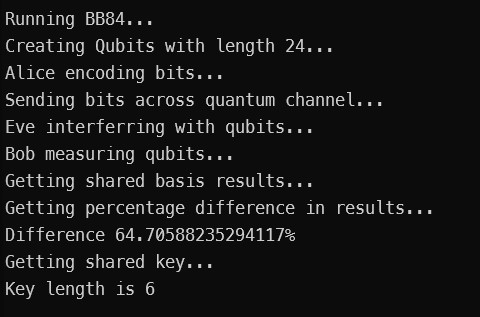
\includegraphics[width=0.3\textwidth]{BB84Output.jpg}


\section{Evaluation}

\section{Conclusions}

\printbibliography

\end{document}

